\section{Speicherhirachie}
	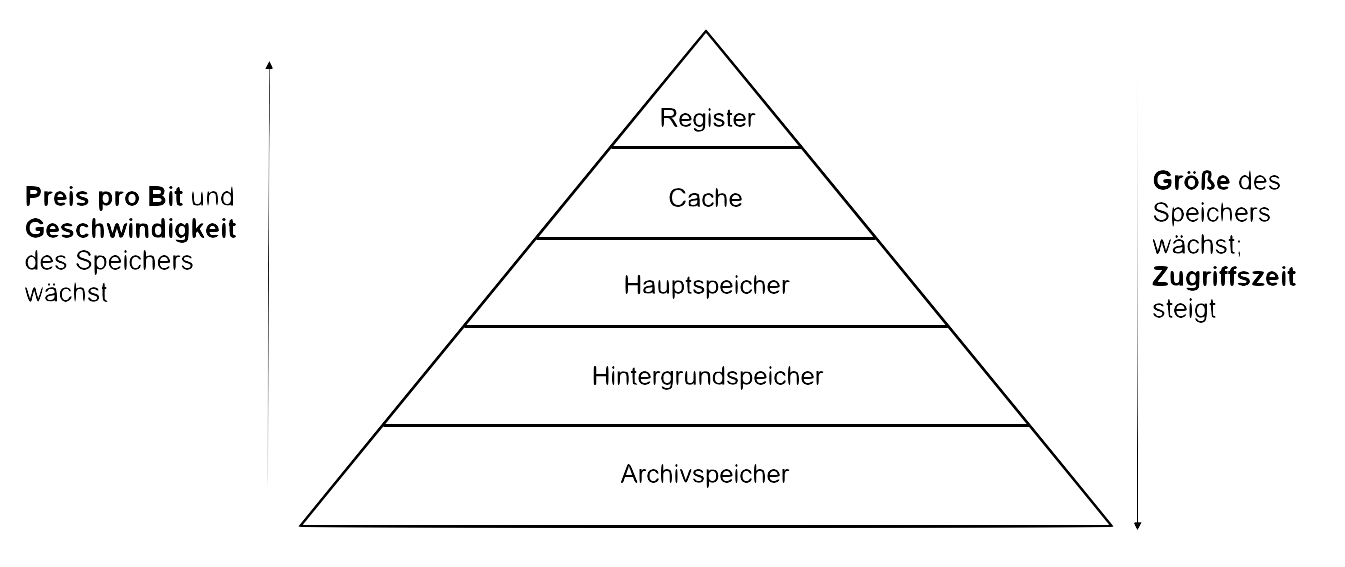
\includegraphics[scale=0.5]{Speicherhierarchie.png}
	\subsection{Performance Gap}
		Die Performanzsteigerung bedeutet, dass die CPU immer mehr Berechnungen in gleicher Zeit ausführen kann. Der Arbeitsspeicher kann ebenfalls mehr Daten in der selben Zeit lesen und weitergeben, jedoch fällt diese Steigerung deutlich geringer aus, was als Performanzlücke bezeichnet wird.
	\subsection{Räumliche und Zeitliche Lokalität}
		\subsubsection{Zeitlich}
			Programme neigen dazu, auf die selbe Adresse innerhalb kürzester Zeit mehrmals zuzugriefen. Chaches nutzen das, indem sie sich Arbeitsspeicherzugriffe merken. Wenn auf eine Adresse mehrmals zugegriffen wird, dann wird der Arbeitsspeicher nur beim ersten Zugriff besucht, anschließend der Cache
		\subsubsection{Räumliche}
			Programme neigen dazu, wenn sie auf eine Adresse X zugreifen, in naher Zukunft auch auf benachbarte Adresse von X zuzugreifen. Caches nutzen das, indem sie bei einem Arbeitsspeicherzugriff automatisch auch die benachbarten Daten (typischerweise etwa 64 Byte) mitladen. Wenn dann kurz darauf ein Zugriff auf eine benachbarte Adresse stattfindet, kann der Cache dieses Datum direkt liefern und muss den Arbeitsspeicher nicht noch einmal anfragen.
			
			